\documentclass[twocolumn,floatfix,nofootinbib,aps]{revtex4-1}
\usepackage[utf8]{inputenc}

\usepackage{amsmath}    % need for subequations
\usepackage{amssymb}    % for symbols
\usepackage{graphicx}   % need for figures
\usepackage{verbatim}   % useful for program listings
\usepackage{color}      % use if color is used in text
\usepackage{subfigure}  % use for side-by-side figures
%\usepackage{hyperref}   % use for hypertext links, including those to external documents and URLs
\usepackage[capitalise]{cleveref}   % use for referencing figures/equations
\begin{document}

\title{Opt-K}
\author{Robert T. McGibbon}
\author{Christian R. Schwantes}
\author{Vijay S. Pande}

\begin{abstract}
Likelihood framework for choosing the optimal number of states in a
Markov State Model
\end{abstract}

\maketitle


\section{Introduction}
\begin{itemize}
\item Many processes in proteins are fundamentally dynamical in nature. Folding, aggregation, cryptic binding sites. Governed by a delicate entropic and enthalpic balance.
\item Set up a conflict between the detailed picture given by MD simulation and the simple picture seen by experiments. Multidimensional time series vs. phenomenological two-state behavior. But sometimes experiments see more complex dynamics too -- interpreted as alternate pathways, kinetic intermediates.
\item Minimially-biased kenetic analysis of MD data has been a challenge for the field. Some procedures, in making strong assumptions about the form of the simplified dynamics -- e.g. rxn coord, G\={o} -- lack the capability to describe the complex systems in which those assumptions break down.
\item Here, we seek to build models that are \emph{suitably} complex, given the data. Markov state models are able to capture both two-state and more complex multi-state kinetics.
\item Like all statistical methods, Markov state models are chacterized by a bias-variance tradeoff. Picking the number of states in the MSM is a key tradeoff parameter, with statistical error balanced against modelling bias.
\end{itemize}

\subsection{Comparison to previous work}
After we've introduced the idea:
\begin{itemize}
\item Contrast with lumping. Instead of going overboard on making too many states and then trying to correct it by merging some of them, we're going to try to pick the right number in the first place.
\item Given the frame that lumping is an attempt to correct the statistical error comping from too many states (bias-variance), it makes sense that spectral methods like PCCA/PCCA+ fail: they're construction assumes that the transition matrix (its eigenspectrum) is known precisely. But the conditions where that is most likely to break down, when there are too many states  -- that's precisely the time that you're trying to apply these methods. So PCCA/PCCA+ is unsuitable here.
\item BACE on the other hand, by explicitly modeling the statistical uncertainty when merging states, does not suffer from this drawback. (say something nice, get greg as reviewer?)
\end{itemize}


\section{Overview}

A significant challenge in the automated construction of Markov state
models is the choice of the number of microstates. Although classical Hamiltonian dynamics form a continuous-time Markov chain in $\mathbb{R}^{6N}$, the Markov property does not hold after the projecting the dynamics onto a basis of discrete indication functions -- the MSM microstates. In particular, when microstates contain within them free energy barriers of substantial magnitude, the validity of the Markov assumption begins to suffer considerably. While this source of modeling error can be addressed by increasing the number of microstates, the reduction in one error comes at the expense of the increase in another. This second source of error is statistical in origin. As the number of states in the model grows, so does the number of parameters required to specify the transition matrix. Because the amount of data is constant, each additional parameter leads to a decrease in the amount of data available per
parameter, which makes the model liable for over-fitting.

Currently, most MSM construction pipelines involve manually selecting the number of microstates. This is done primarily by human intuition, guided by the Chapman–Kolmogorov test, and is a significant bottleneck.

Here, we introduce a new procedure for scoring the likelihood of an MSM, which, together with the Bayesian information criterion (BIC), enables the optimal selection of both the number of states and clustering algorithm.

Within the discrete state space, the likelihood of an ensemble of
trajectories given the MSM is straightforward. It is computed simply by taking the product of the state to state transition probabilities along the path.
These state-to-state transition probabilities are entries in the MSM's so-called transition matrix, and are the central parameters of the model. However, as we vary the number of states, it is not permissible to simply compare these likelihoods to select an optimal number of states. Doing so, the optimal model would always be the trivial model, with only one state, as the transition probability in that model would be $1$ and thus the likelihood of any trajectory within that state space would be $1$.

The proper likelihood is not of the trajectory within the discrete state
space; instead it is the likelihood of the trajectory within the
continuous phase space, on which the discrete states are merely an
indicator function basis. 

\begin{equation}
P[X_{0...T-1}] dx^T = \prod_{i=0}^{T-1} T(X_i \rightarrow X_{i+1}) \cdot \prod_{i=0}^{T} p(X_{i} | \sigma(X_{i}))
\label{eq:like}
\end{equation}

With a discrete, non-overlapping state space, the likelihood of the
trajectory can be decomposed into a product over the trajectory of two
types of terms: the state to state transition probabilities and the
``emission'' probabilities of each state, the probability of observing a
conformation at a given location in phase space given that the
conformation, $x_t$, is within a certain state, $\sigma(x_t)$.

\section{Emission Distributions}

Up until this point, the emission probability distributions have not
been a model parameter for MSMs. Nevertheless, they are a critical
parameter for evaluating trajectory likelihoods. For example, consider two MSMs with the same transition probabilities. However, in one case, the emission distributions for each state are highly peaked at specific locations in phase space, whereas in the other model the emission distributions are uniform over the volume of the clusters. If the trajectory actually does go through the first models' regions of high likelihood, it would be clear that the first model more accurately fits the data.

However, the long timescale behavior of the MSM, the quantity of most
interest scientifically, is independent of the choice of the emission
distributions. It is only determined by the eigenspectrum of the
transition matrix elements. The emission distributions determine the
estimated eigenfunctions, but not the eigenvectors.

Therefore, the most appropriate emission distribution for discrete state
MSMs is that of the uniform distribution over the phase-space volume of
the state. That is, the likelihood of observing a conformation in phase
space given that the conformation is assigned to state $i$ is $0$
if the conformation is outside of the bounding volume of the state and
constant if the conformation is within the volume. This constant is set
so that the distribution integrates to $1$, and is thus the reciprocal
volume of the microstate.

% \begin{align*}
% p(x | s) &= C \\
% \int p(x | s) dx &= 1 \\
% \int C \mathbf{1}_s dx &= 1 \\
% C &= \frac{1}{\int \mathbf{1}_s dx}
% \end{align*}

\begin{equation}
\label{eq:like_vol}
P[x_{0...T-1}] dx^T = \prod_{i=0}^{T-1} T(x_i \rightarrow x_{i+1}) \cdot \prod_{i=0}^T \frac{1}{V_{\sigma(x_{i})}}
\end{equation}

\section{Algorithm}

To use this uniform distribution emission model, computationally, we
need to compute the volume of our MSM states, which are high-dimensional
Voronoi cells. While trivial in two or three dimensions, this
computational geometry task becomes challenging in large dimensional
settings. The computation of high dimensional volumes has occupied significant
attention in recent years in the computational geometry literature, especially
via randomized algorithms.\cite{Simonovits03, Lovasz03}

A further challenge is the procedure by which to model the volume of states which are at the ``edge'' of the MSM, whose Voronoi cells extend to infinity in some direction. Is the volume of these states unbounded? It is appropriate to assert that the volume of these edge states is bounded in some way by the extent of our dataset. For example, the volume of a state might be defined as the volume of the intersection of its Voronoi cell and the convex hull of the whole dataset, which would encode the assumption that the likelihood of points
outside the convex hull of the sampled data is vanishing.

We use a slightly modified version of this definition that adopts
the same spirit. Instead of taking the outer bounding envelope to be the convex hull of the data, we take it to be the set of all trial points such that the nearest sampled configuration to the trial point is closer than a certain cutoff, $R$. This can be computed relatively efficiently using a Balltree data structure.\cite{Omohundro1989} For further efficiency, it is feasible to use only a random subsample of the dataset for this nearest neighbor computation.

Instead of computing the volume of the Voronoi cells explicitly, we instead
compute the ratio of volume of each Voronoi cell to the volume of the
bounding envelope. Because the bounding envelope's volume is independent of the clustering parameters, its inclusion changes all of the calculated likelihoods by a constant multiplicative factor, and can thus be discarded from the perspective of model comparison.

To compute the fractional volumes of the Voronoi cells, we utilized a randomized algorithm, as exact algorithms have an impermissible exponential time complexity with respect to the dimensionality. First, we generate points inside of the bounding region using a lazy random walk Markov chain Monte Carlo algorithm.\cite{Kannan97} This random walk converges to sampling from the uniform distribution over the interior. After a sufficient burn in period, for each sampled point we compute its nearest MSM state center, assigning it to that state. As the number of randomly sampled points goes to infinity, the fraction of the points assigned to each state converges to being proportional to the state's volume.

This algorithm is highly amenable to parallel computation.

\section{Validation}

\subsection{Langevin Dynamics on the M\"uller Potential}
We being by using the procedure described above on simulated Langevin dynamics on the M\"{u}ller potential (\cref{fig:muller_pot}). This data was clustered into models of different sizes using one of two algorithms. The first, K-Centers, tends to make equal sized states as it works to minimize the maximum distance between a conformation and its generator. The second, Hybrid, will make varying size states because it works to minimize the average distance between conformations and their generators. In both cases, we built models ranging from 50 to 1,000 total states. Since this space is only two-dimensional, we used simple rejection sampling to compute the volumes. 

Briefly, we generated uniform random vectors within a bounding box whose size was slightly larger than the data. This random sample was then accepted if it was 'close enough' to a generator in the 100 state model, where close enough meant it was within 0.2 units from any generator in that model. This was used to approximate the convex hull of the data. Then the accepted points were assigned to a state. Then the volume of a state is proportional to the number of samples assigned to that state divided by the total number of samples. %We note, that these volumes are actually in units of the total acceptable volume. This affects the absolute value of the likelihood, however, since the total volume was constant in all cases, the relative likelihoods are the same.
\begin{figure}[h!]
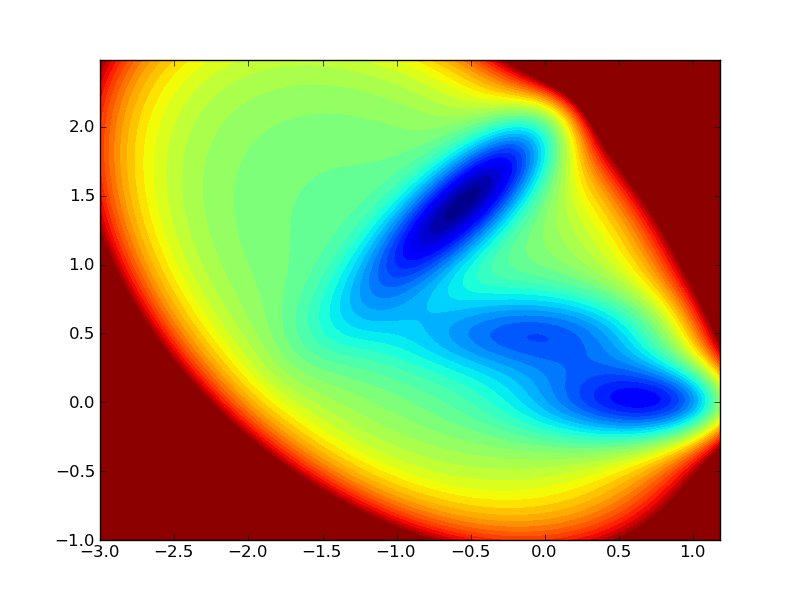
\includegraphics[width=2in]{figs/muller_pot.png}
\caption{The M\"{u}ller potential consists of three metastable wells. We simulated Langevin dynamics on this potential as a validation of the new likelihood function.}
\label{fig:muller_pot}
\end{figure} 

We built an MSM using a fixed lag time for each state decomposition and then calculated the likelihood according to \cref{eq:like_vol}. These likelihoods increased rapidly with $k$, but then plateaued at a value of around 300 states \cref{fig:like_kcenters}. At this plateau, we can conclude that we do not gain any new information by adding new states to our model, to compensate for the additional parameters. This is a heuristic argument that can be made more rigorous with the introduction of model comparison metrics like the Bayesian information content (BIC), which is defined in \cref{eq:bic}.

\begin{equation}
BIC = -2 \log L + m \log(n) 
\label{eq:bic}
\end{equation} Here, $L$ denotes the likelihood of a model, while $m$ is the number of parameters used in the model, and $n$ is the number of data points. While somewhat heuristic, the BIC can be viewed as an approximation to the Bayes Factor, whose direct computation involves the infeasible task of integrating over the posterior distribution of Markov models.

We found that the BIC of the models built using K-Centers clustering has a minimum at $k=250$. This minimum is the ``optimal'' model according to the BIC. As an orthogonal check on the selection of this minimum, we plotted the three slowest implied timescales in the models as a function of $k$. Because the model's implied timescales are estimators of the eigenvalues of the underlying potential's transfer operator, their invariance with respect to the number of states is a standard check on model quality. The optimal model was close to the point at which the implied timescales became constant. 

\begin{figure}
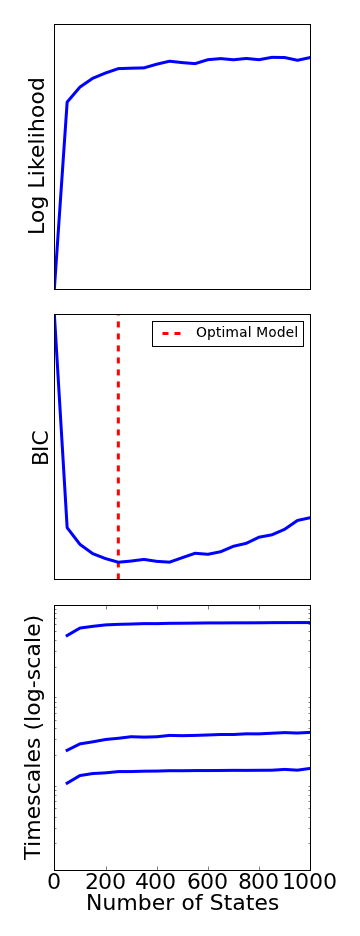
\includegraphics[width=2in]{figs/like_comp.png}
\caption{For models built between 50 and 1,000 states using the K-Centers algorithm, the log likelihood function increased quickly and plateaued at approximately 300 states. Heuristically, at this point, adding another state does not add anything to the model. As a result, by using a criterion, like the BIC, that penalizes using additional parameters to fit the data, we can find an ``optimal'' model. Interestingly, the BIC optimal model occurs at 250 states, which also corresponds to where the three slowest timescales plateau.}
\label{fig:like_kcenters}
\end{figure}

\begin{figure*}
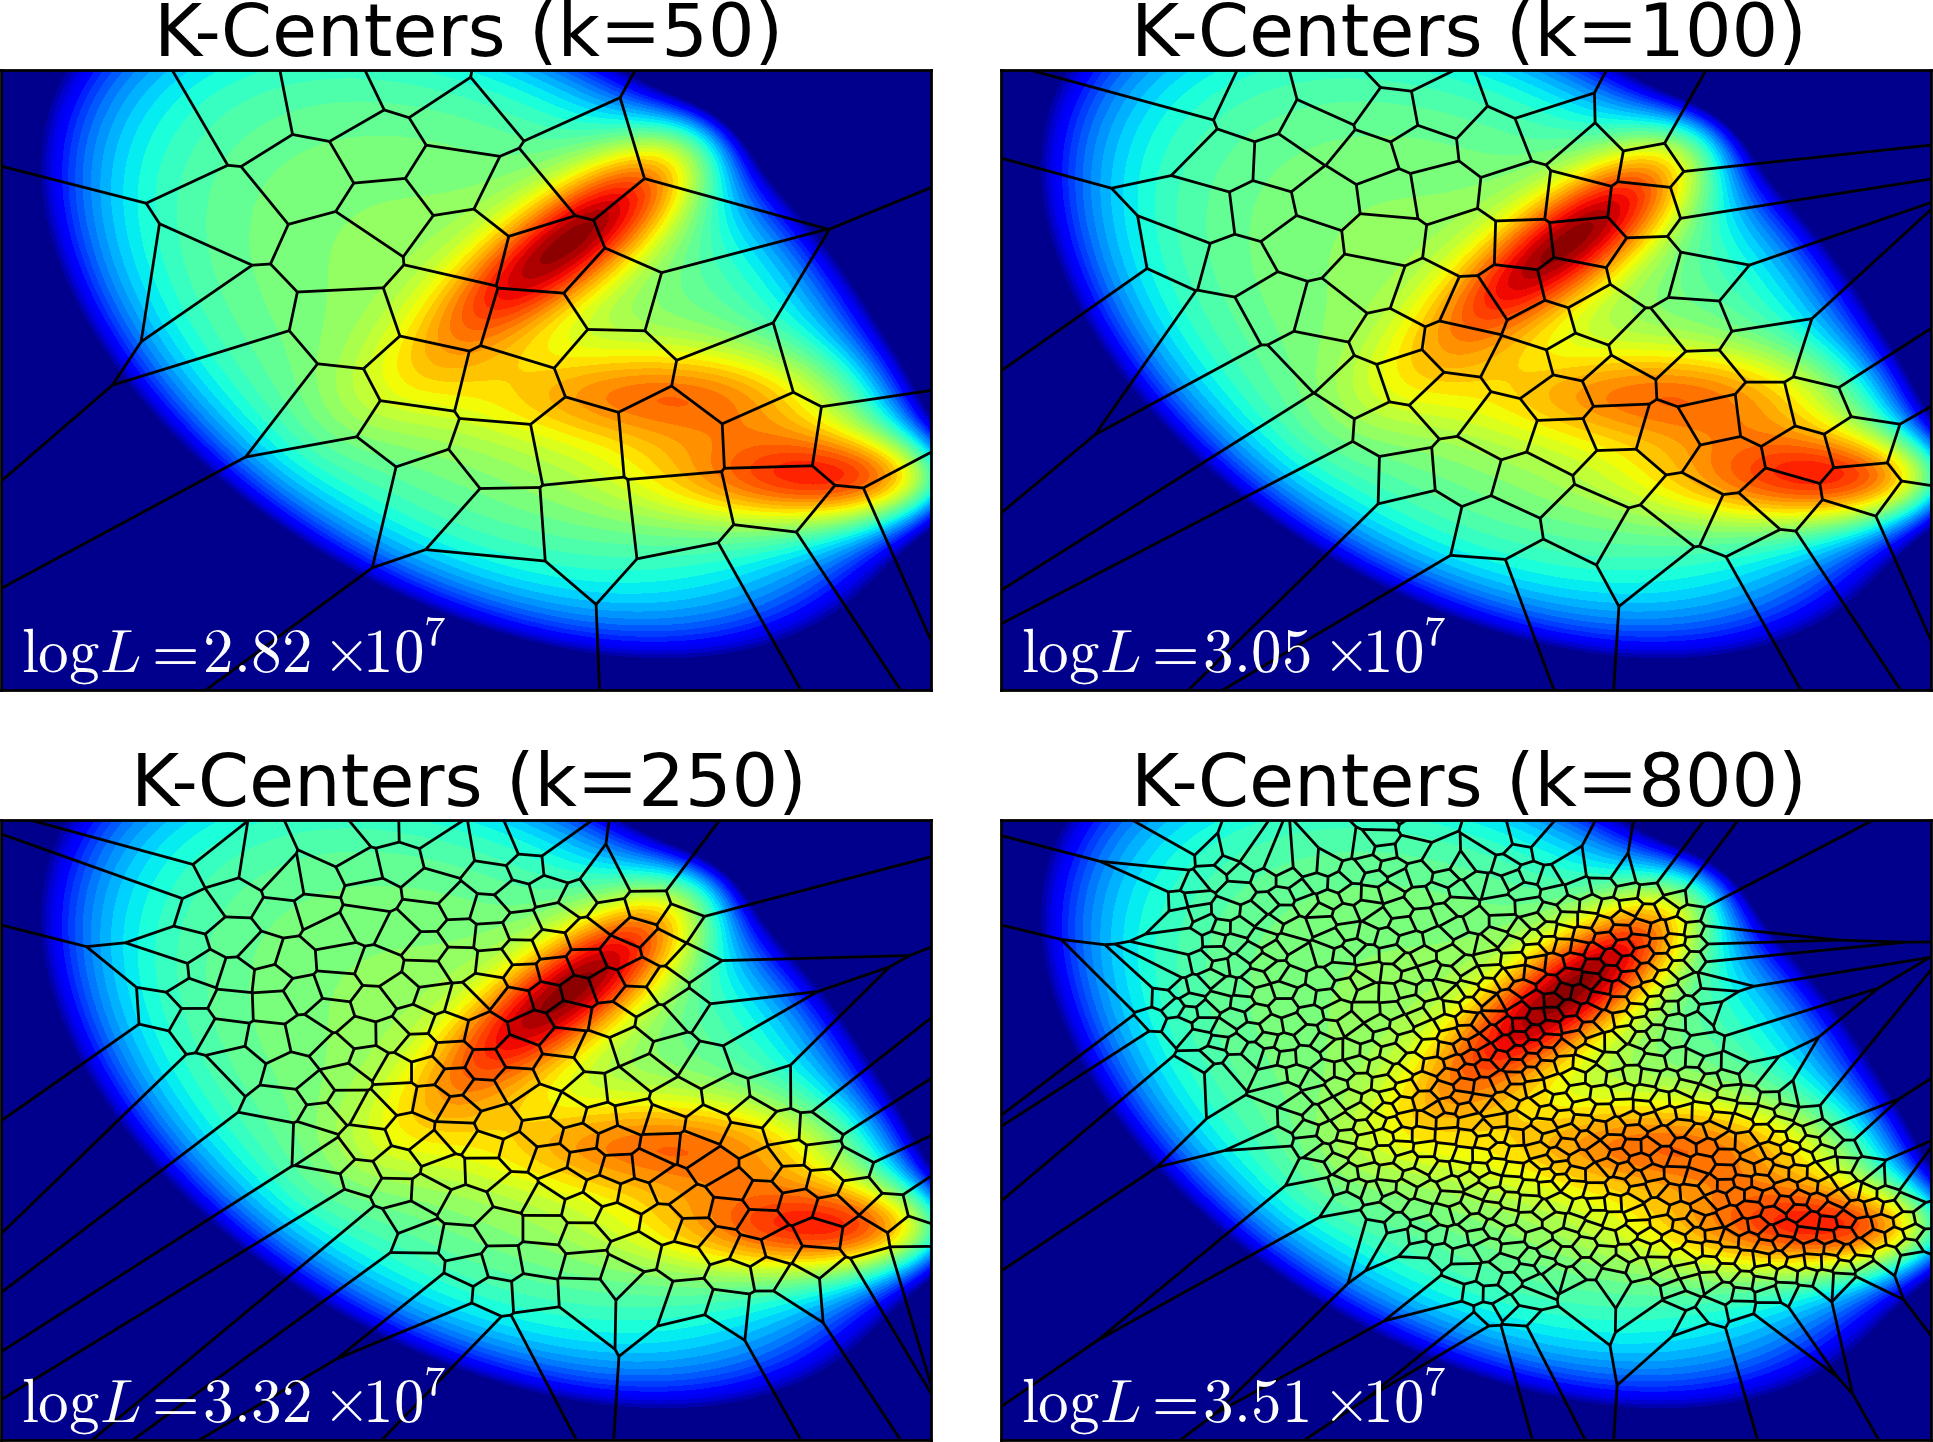
\includegraphics[width=5in]{figs/kcent_vors.png}
\caption{For K-Centers models, we observed a rapid increase in likelihood followed by a plateau. For models built with too few states, the states within the metastable wells are too large. By increasing the number of states, the resolution in increased, but using too many states leads to a model like the bottom right which is clearly over-fit and so has a non-optimal BIC despite having a higher likelihood.}
\end{figure*}

\begin{figure}
\centering
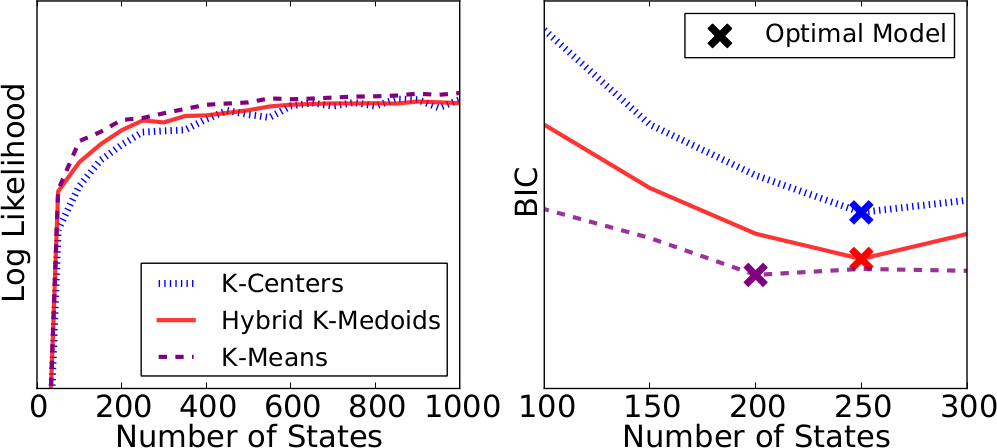
\includegraphics[width=3.4in]{figs/cluster_comp.png}
\caption{We also compared three clustering algorithms and used the likelihood function to determine which is best. The likelihood of the K-Means models was always larger than the other two. Additionally, the K-Means algorithm plateaued at a lower value of $k$, which corresponded to a minimum in the BIC curve at 200 states vs. the optimal models of 250 states in the K-Centers and Hybrid K-Medoids models.} \end{figure}

\begin{figure}
\centering
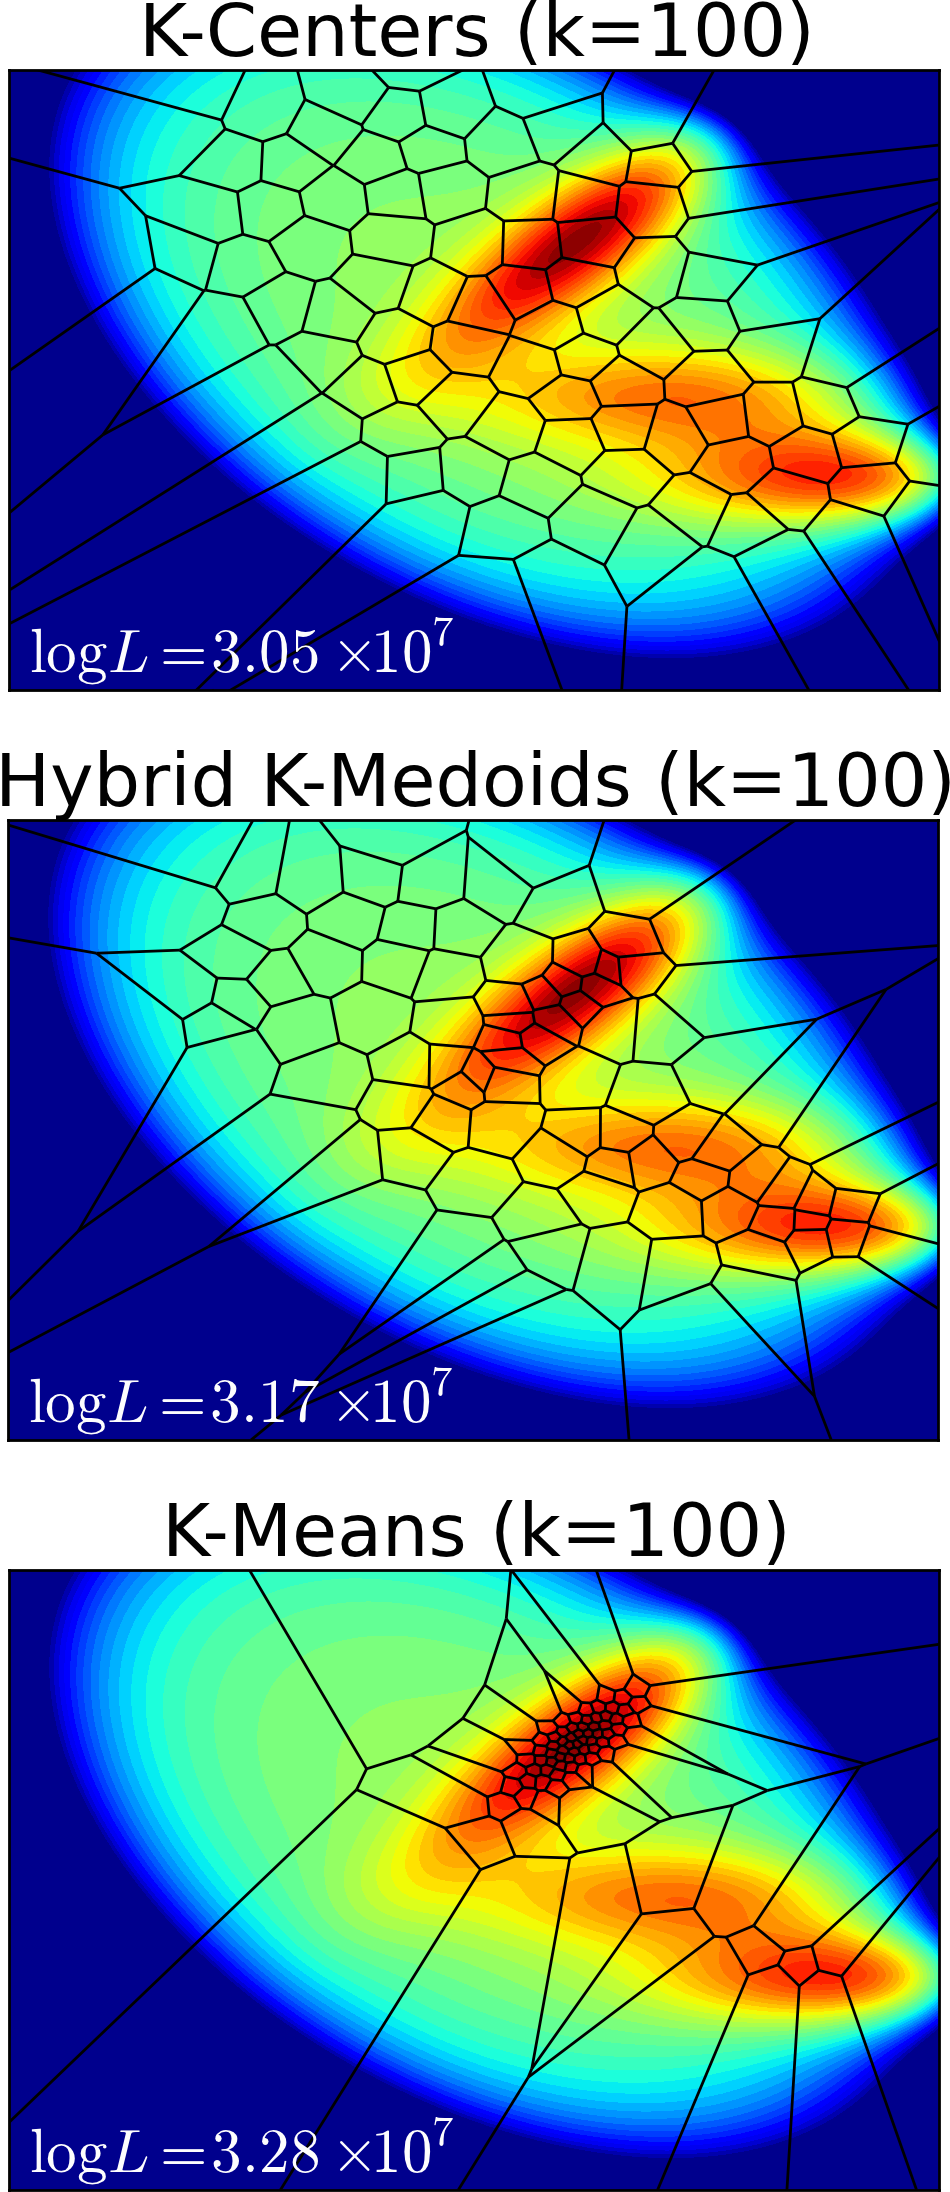
\includegraphics[width=2in]{figs/clust_vors.png}
\caption{The likelihoods (and BIC's) of the three clustering algorithms predicted that the K-Means algorithm is the better clustering algorithm. The result of K-Means is many states clustered into the highest density areas of the potential. The Hybrid K-Medoids ends up somewhere in between the K-Centers model and the K-Means model. This is likely due to the implementation being an approximate algorithm that requires more iterations to converge to the best state decomposition.}
\end{figure}

\begin{figure}
\centering
%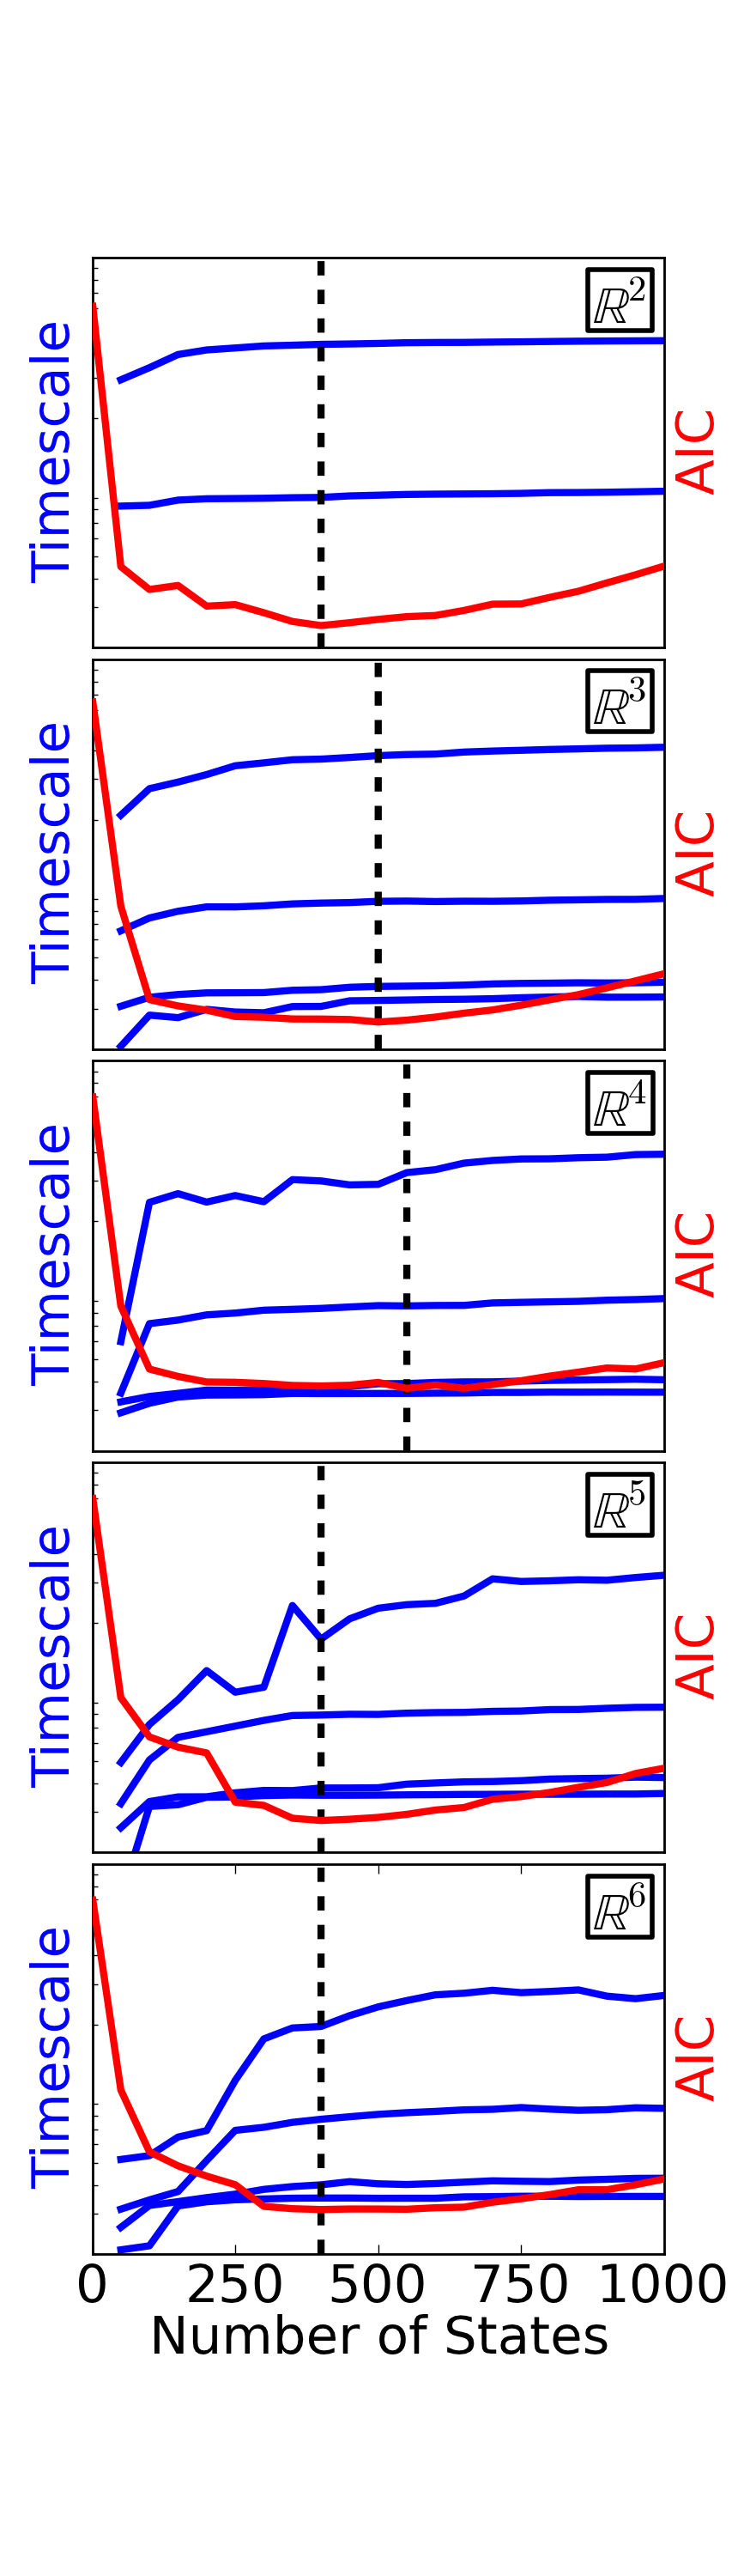
\includegraphics[width=2in]{figs/ww_aic_vs_eval.png}
% Include the AIC in an SI section discussing the BIC vs AIC vs etc.
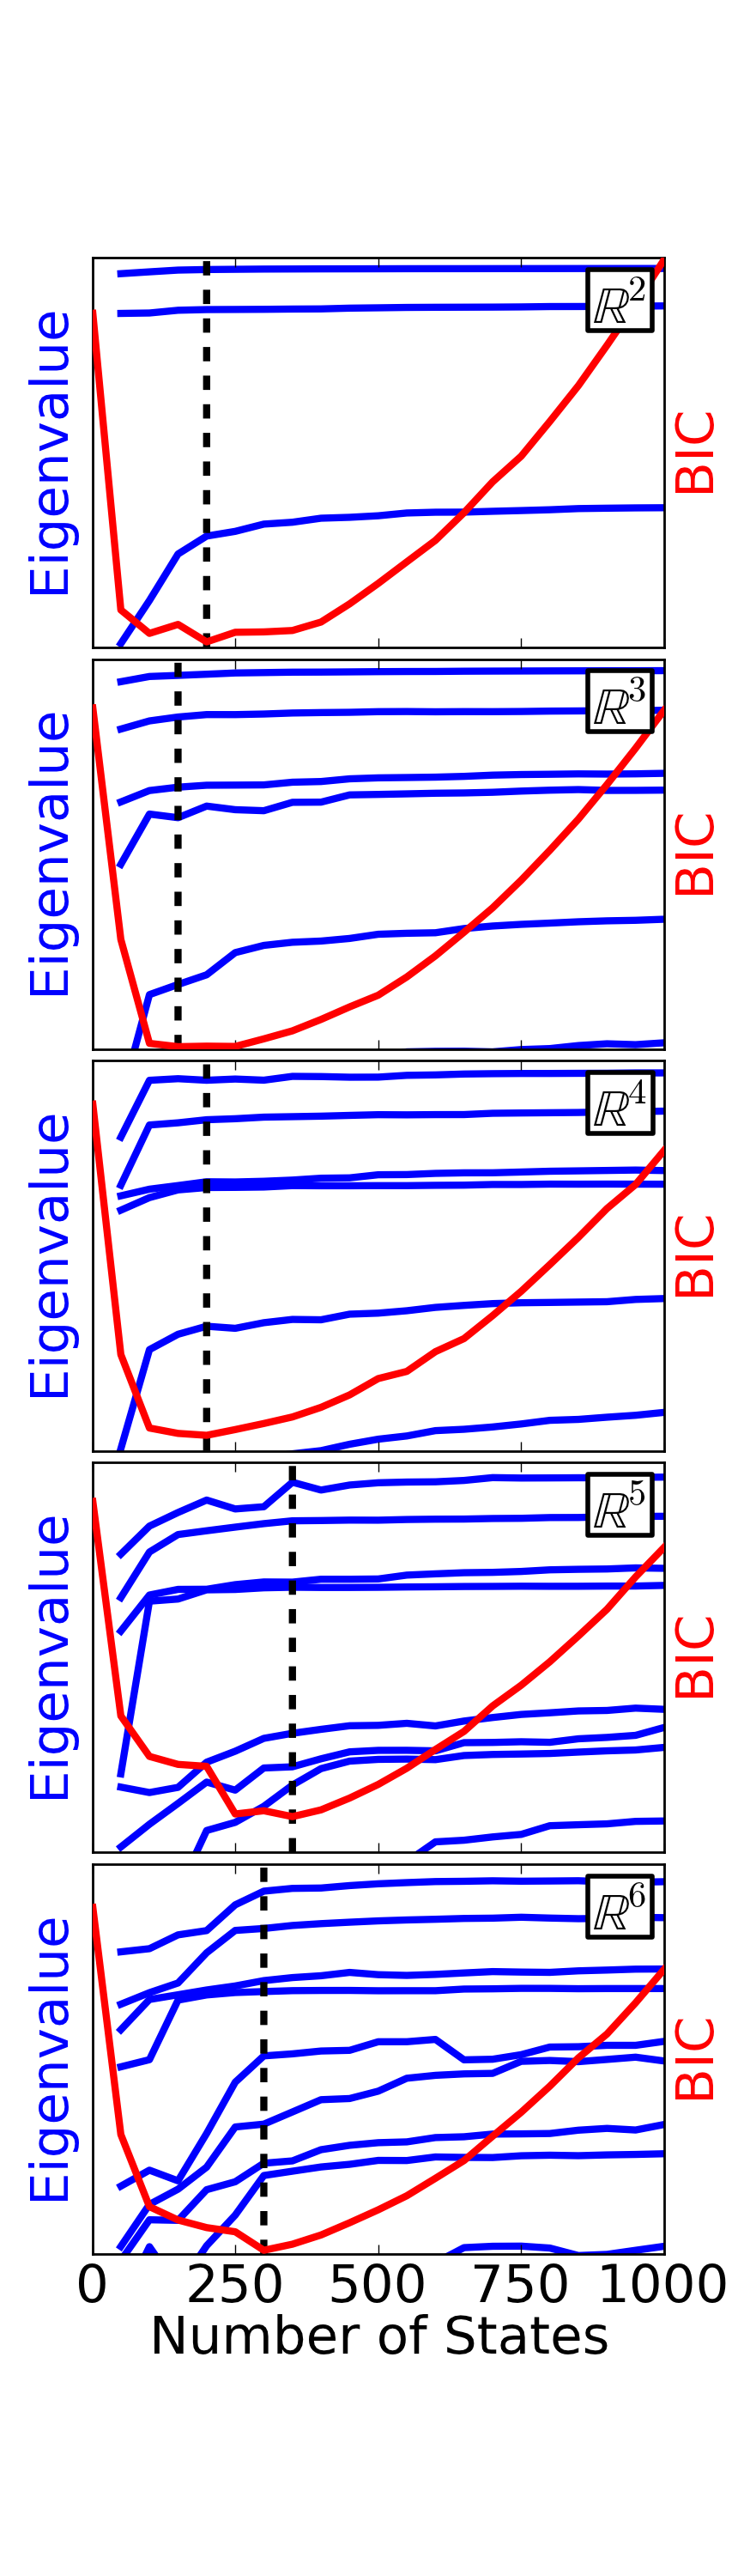
\includegraphics[width=2in]{figs/ww_bic_vs_eval.png}
\caption{In the WW domain simulations, we projected the coordinates into reduced spaces from two to six dimensions, using tICA \cite{Schwantes:2013..}. The AIC optimal models were in the 200 to 400 state range. We compared the AIC with the autocorrelation convergence, and found that the AIC optimal model coincided generally with the point at which the autocorrelation functions converged. The BIC, penalizes the models more, and so gave rise to BIC optimal models between 100 and 300 states.}
\end{figure}

\bibliography{bibliography}
\end{document}
